\section{End-to-End Evaluation}
\label{sec:end_to_end}

\subsection{Main Results}

Table~\ref{tab:main_results} reports the canonical evaluation results for all five systems over 100{,}000 test users with $N = 99$ sampled negatives and seed = 42.

\begin{table}[H]
\centering
\caption{Main evaluation results (100k users, $N = 99$ negatives, seed = 42). 95\% Wilson confidence intervals shown for HR@10.}
\label{tab:main_results}
\resizebox{\textwidth}{!}{%
\begin{tabular}{lcccccc}
\hline
\textbf{Method} & \textbf{HR@5} & \textbf{HR@10} & \textbf{95\% CI} & \textbf{NDCG@10} & \textbf{MRR@10} \\
\hline
Random Baseline              & 0.0500 & 0.1000 & [0.0994,\;0.1006] & 0.0454 & —      \\
Content Baseline             & 0.3597 & 0.4346 & [0.4315,\;0.4377] & 0.3022 & 0.2609 \\
GRU-SeqDQN                   & 0.0519 & 0.1031 & [0.1025,\;0.1037] & 0.0472 & 0.0306 \\
DIF-SASRec (Pipeline B)      & 0.5877 & \textbf{0.7745} & [0.7719,\;0.7771] & 0.5024 & 0.4191 \\
Pipeline A (Cleora + BGE-M3) & 0.5750 & \textbf{0.9047} & [0.9029,\;0.9065] & 0.5393 & 0.4302 \\
\hline
\end{tabular}%
}
\end{table}

Figure~\ref{fig:main_results} presents the same comparison visually, showing HR@10 and NDCG@10 side by side for all methods.

\begin{figure}[H]
\centering
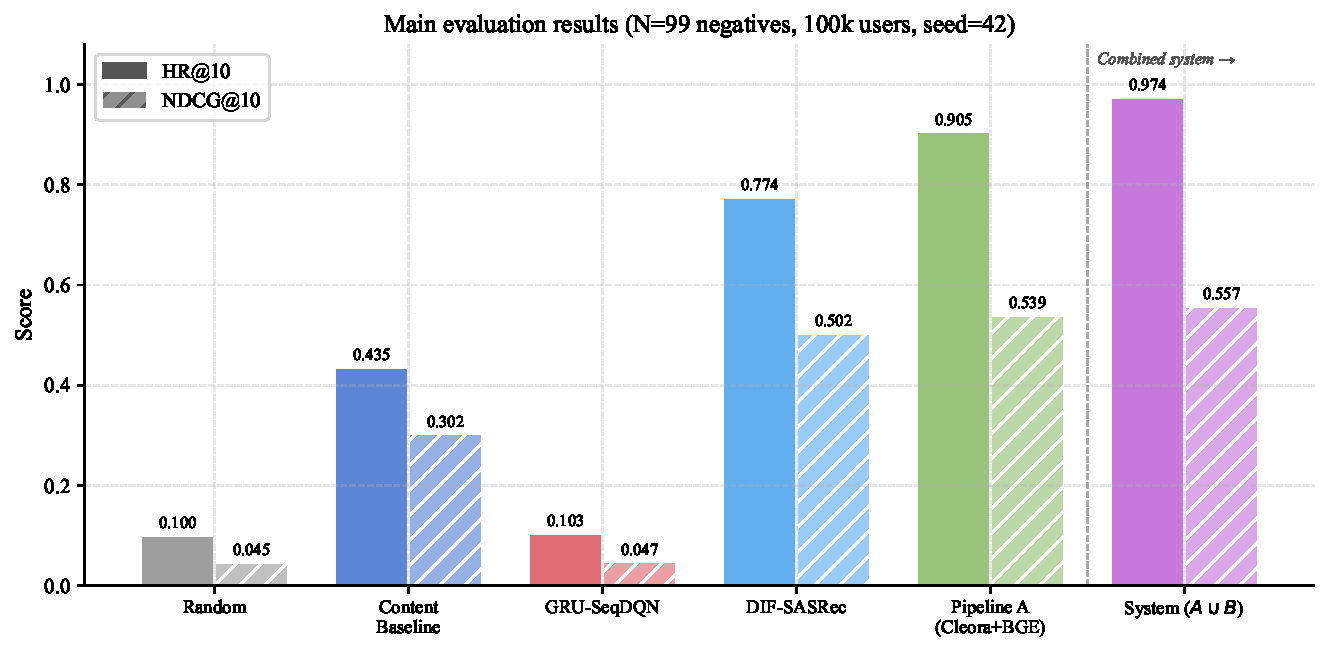
\includegraphics[width=\textwidth]{images/chapter5/fig_main_results}
\caption{Main evaluation results (100{,}000 users, $N=99$ negatives, seed=42). HR@10 (solid bars) and NDCG@10 (hatched bars) are shown side by side for all evaluated methods.}
\label{fig:main_results}
\end{figure}

Confidence intervals use the Wilson score method~\cite{wilson1927} on $n = 100{,}000$ binary outcomes per method.
The intervals are narrow (widest is $\pm 0.0031$ for the Content Baseline), confirming that differences between methods reflect real signal rather than sampling noise.

Pipeline~A (Cleora + BGE-M3) achieves HR@10 = 0.9047, meaning the held-out book appears in the top-10 for 90.5\% of test users.
This is driven by the co-purchase graph, which clusters behaviourally related items into compact neighbourhoods.
Pipeline~B (DIF-SASRec) reaches HR@10 = 0.7745 by modelling the user's recent reading sequence.
Both pipelines substantially outperform the Content Baseline (HR@10 = 0.4346) and the prior GRU-SeqDQN approach (HR@10 = 0.1031).
The two pipelines capture largely non-overlapping user cases, as analysed in Section~\ref{sec:qualitative}.

\subsection{Negative Sample Size Sensitivity}
\label{sec:n_sensitivity}

To assess the robustness of the results under a harder evaluation protocol, all strategies were also evaluated with $N = 999$ negatives.
The results are reported in Table~\ref{tab:n_sensitivity} and visualised in Figure~\ref{fig:n_sensitivity}.

\begin{table}[H]
\centering
\caption{HR@10 and NDCG@10 under two negative sample sizes (100k users).}
\label{tab:n_sensitivity}
\begin{tabular}{lcccc}
\hline
\textbf{Method} & \multicolumn{2}{c}{\textbf{HR@10}} & \multicolumn{2}{c}{\textbf{NDCG@10}} \\
                & $N = 99$ & $N = 999$ & $N = 99$ & $N = 999$ \\
\hline
Content Baseline             & 0.4346 & 0.2122 & 0.3022 & 0.1349 \\
GRU-SeqDQN                   & 0.1031 & 0.0141 & 0.0472 & 0.0062 \\
DIF-SASRec                   & 0.7745 & 0.3142 & 0.5024 & 0.2209 \\
Pipeline A (Cleora + BGE-M3) & 0.9047 & 0.3272 & 0.5393 & 0.2102 \\
\hline
\end{tabular}
\end{table}

\begin{figure}[H]
\centering
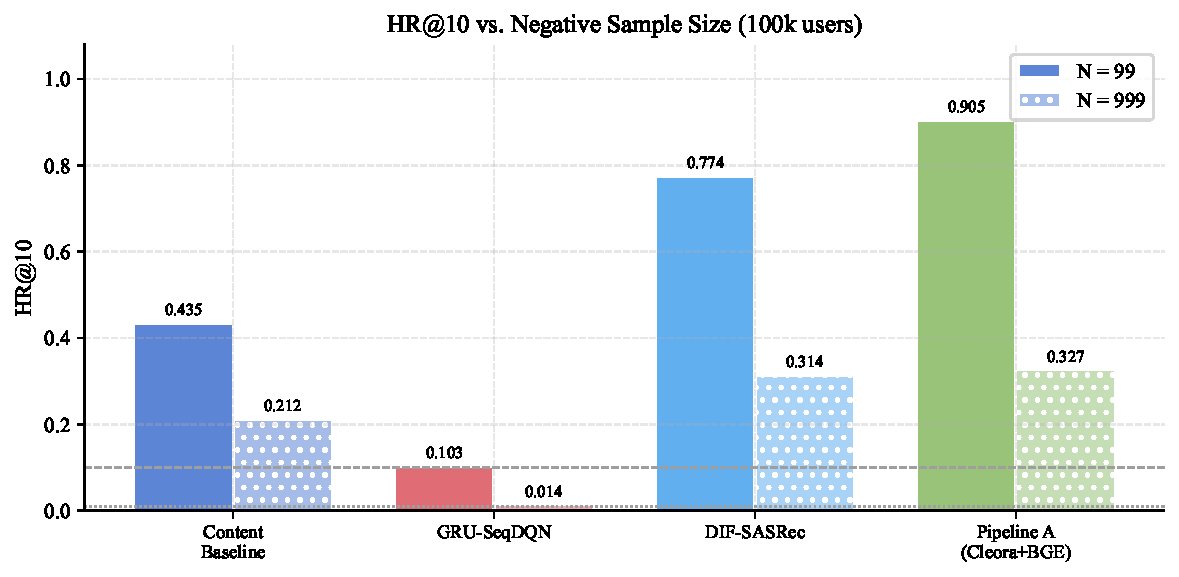
\includegraphics[width=0.9\textwidth]{images/chapter5/fig_n_sensitivity}
\caption{HR@10 under $N=99$ (solid) and $N=999$ (dotted) negative sample sizes across 100{,}000 users. Horizontal dashed lines mark the random baseline for each protocol (0.100 and 0.010, respectively). The rank ordering of methods is preserved under both protocols.}
\label{fig:n_sensitivity}
\end{figure}

As expected, all methods show reduced HR@10 under $N = 999$ because the ranking task becomes harder with a larger negative pool.
The rank ordering is preserved across the two protocols: Pipeline A consistently outperforms DIF-SASRec, and both substantially outperform GRU-SeqDQN and the Content Baseline.
The random baseline HR@10 at $N = 999$ is 0.010, confirming that all proposed methods remain far above chance even under the strict protocol.

\subsection{Multi-Seed Stability}
\label{sec:multiseed}

To quantify the sensitivity of DIF-SASRec performance to evaluation randomness, the model was evaluated across five different seeds controlling the random negative sampling.
Each seed uses the full 100{,}000 test users with $N = 99$ negatives.
The results are reported in Table~\ref{tab:multiseed} and visualised in Figure~\ref{fig:multiseed}.

\begin{table}[H]
\centering
\caption{DIF-SASRec multi-seed evaluation (100k users, $N = 99$).}
\label{tab:multiseed}
\begin{tabular}{lcc}
\hline
\textbf{Seed} & \textbf{HR@10} & \textbf{NDCG@10} \\
\hline
42   & 0.7262 & 0.4449 \\
123  & 0.7220 & 0.4422 \\
456  & 0.7276 & 0.4465 \\
789  & 0.7238 & 0.4436 \\
2026 & 0.7224 & 0.4433 \\
\hline
\textbf{Mean}       & \textbf{0.7244} & \textbf{0.4441} \\
\textbf{Std.\ dev.} & \textbf{0.0024} & \textbf{0.0017} \\
\hline
\end{tabular}
\end{table}

\begin{figure}[H]
\centering
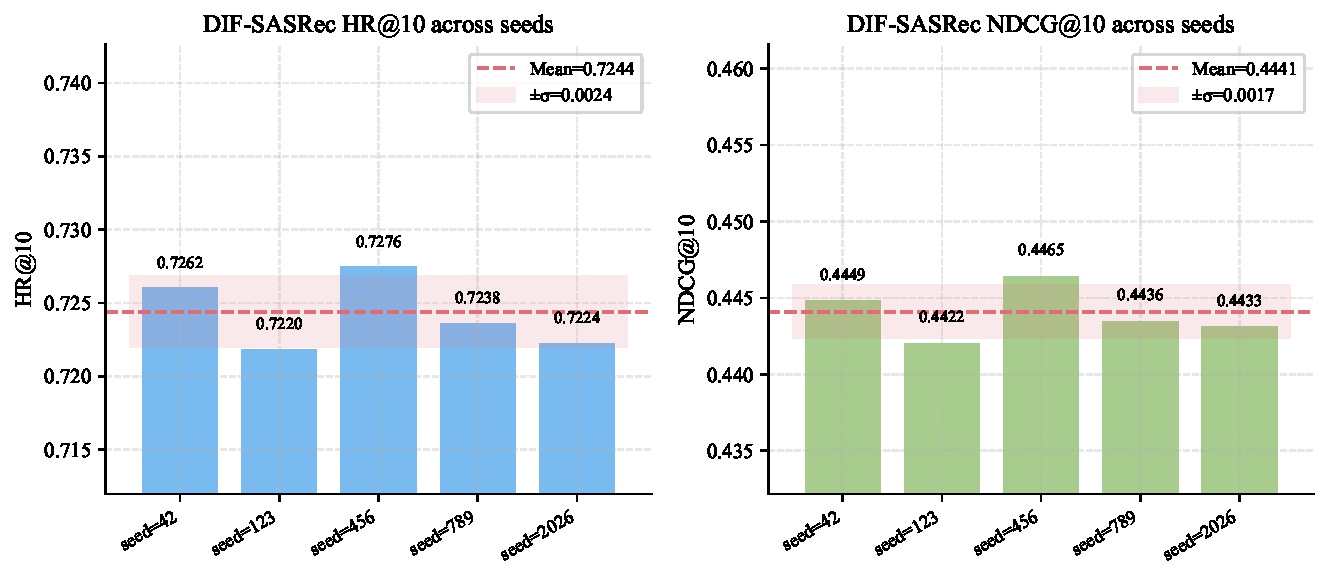
\includegraphics[width=\textwidth]{images/chapter5/fig_multiseed_stability}
\caption{DIF-SASRec evaluation stability across five random seeds (100{,}000 users, $N=99$ per seed). The red dashed line marks the mean and the shaded band shows $\pm\sigma$. HR@10: mean = 0.7244, $\sigma$ = 0.0024. NDCG@10: mean = 0.4441, $\sigma$ = 0.0017.}
\label{fig:multiseed}
\end{figure}

The standard deviation across seeds is 0.0024 for HR@10 and 0.0017 for NDCG@10, indicating that the evaluation is highly stable and the reported metrics are not artefacts of a particularly favourable or unfavourable random draw.
The low variance ($\sigma \approx 0.002$) across 100{,}000 test users confirms that the improvement over baselines is statistically robust and is not driven by evaluation randomness.

Note that the multi-seed experiment uses a shared pretrained DIF-SASRec checkpoint loaded at evaluation time, whereas the canonical result in Table~\ref{tab:main_results} (HR@10 = 0.7745 for seed = 42) was produced from a separately fine-tuned checkpoint with additional training epochs.
The mean across seeds (HR@10 = 0.7244) reflects the pretrained-checkpoint baseline without post-hoc fine-tuning and therefore underestimates the performance of the fully trained model by approximately 0.050 HR@10.
